\chapter{内分泌系统疾病}

\chapterabstract{本章介绍了单纯性甲状腺肿、弥漫性毒性甲状腺肿、甲状腺肿瘤、糖尿病等常见内分泌疾病,要求掌握单纯性甲状腺肿、弥漫性毒性甲状腺肿、糖尿病的概念和病理变化;熟悉甲状腺肿瘤的常见类型及其病理变化;能联系弥漫性毒性甲状腺肿的病因、病理变化与临床表现之间的关系。}

内分泌系统(endocrine
system)包括内分泌腺、内分泌组织(如胰岛)和散在于各系统或组织内的内分泌细胞。内分泌系统与神经系统共同调节机体的生长发育和代谢,维持体内平衡或稳定。由内分泌腺或散在的内分泌细胞所分泌的高效能的生物活性物质,经组织液或血液传递而发挥其调节作用,此种化学物质称为激素(hormone)。按激素的化学性质可分为含氮激素和类固醇激素两大类,前者主要在粗面内质网和高尔基复合体内合成,其分泌颗粒有膜包绕;后者在滑面内质网内合成,不形成有膜包绕的分泌颗粒。激素传递的方式主要有:①远距离分泌(telecrine):激素释放后直接进入毛细血管,经血液运输至远距离的靶细胞组织而发挥作用,大多数激素的传递采用这种传递途径发挥作用;②旁分泌(paracrine):某些激素可不经血液运输,仅由组织液扩散而作用于邻近细胞,这种方式称为旁分泌;③自分泌(autocrine):有的作用于分泌激素细胞的本身,称为自分泌;④胞内分泌(endocellular
secretion):还有的内分泌细胞的信息物质不分泌出来,原位作用该细胞浆内的效应器上,称为胞内分泌。

内分泌系统的组织或细胞发生病变,如增生、肿瘤、炎症、血液循环障碍、遗传等疾病均可引起激素分泌增多或减少,导致功能的亢进或减退,使相应靶组织或器官增生、肥大或萎缩。内分泌系统疾病很多,本章主要介绍部分常见、多发的内分泌系统疾病。

\begin{framed}
{案例12-1}

{【病例摘要】}

患者,女,28岁,因心悸、多汗怕热、食欲增加、消瘦、双眼球前突,来我院就诊入院。体格检查:体温37.3℃,脉搏104次/分,呼吸20次/分。双侧甲状腺弥漫性对称性肿大,可闻及血管杂音。双眼球前突,手掌心潮湿,有明显的手震颤。心尖区第一心音亢进。实验室检查:血清游离三碘甲状腺原氨酸(FT3)37
pmol/L,血清游离甲状腺素(FT4)19 pmol/L,TRH兴奋实验无反应。

正常值:体温36.5~37.5℃,脉搏60~100次/分,呼吸16~20次/分,血压90~140/60~90
mmHg,FT3 9~25 pmol/L,FT4 3~9 pmol/L。

{【问题】}

(1)该病人患何种疾病?诊断依据是什么?

(2)主要脏器可能有何病变?
\end{framed}

\section{甲状腺疾病}

\subsection{单纯性甲状腺肿}

单纯性甲状腺肿(simple goiter)亦称弥漫性非毒性甲状腺肿(diffuse
nontoxic
goiter),是以缺碘、致甲状腺肿物质或相关酶缺陷等原因所致的甲状腺素分泌不足,促甲状腺素(TSH)分泌增多,甲状腺滤泡上皮增生,滤泡内胶质堆积而使甲状腺代偿性肿大,不伴有明显的甲状腺功能亢进或减退。本型甲状腺肿常常是地方性分布,又称地方性甲状腺肿(endemic
goiter),也可为散发性。据报道,目前全世界约有10亿人生活在碘缺乏地区,我国病区人口超过3亿,大多位于内陆山区及半山区,全国各地均有散发。本病主要表现为甲状腺肿大,不伴有肿瘤和炎症,病程初期甲状腺多为弥漫性肿大,以后可发展为多结节性肿大。一般无临床症状,部分病人后期可引起压迫、窒息、吞咽困难和呼吸困难,少数患者可伴甲状腺功能亢进或低下等症状,极少数可癌变。

\subsubsection{病因及发病机制}

大多数单纯性甲状腺肿患者没有明显的病因,部分患者的发病可能与下列因素有关:

\paragraph{碘缺乏}
碘是合成甲状腺激素的必需元素,地方性水、土、食物中缺碘及机体青春期、妊娠和哺乳期对碘需求量增加而相对缺碘,机体不能合成足够的甲状腺激素,反馈刺激垂体TSH分泌增多,甲状腺滤泡上皮增生,摄碘功能增强,达到缓解。如果持续长期缺碘,一方面滤泡上皮增生,另一方面所合成的甲状腺球蛋白没有碘化而不能被上皮细胞吸收利用,则滤泡腔内充满胶质,使甲状腺肿大。用碘化食盐和其他富含碘的食品可治疗和预防本病。我国是碘缺乏严重的国家,国家推行的“全民加碘盐”政策是防止碘缺乏病的最有效的措施。

\paragraph{致甲状腺肿物质的作用}
①水中大量钙和氟可引起甲状腺肿,因其影响肠道碘的吸收,且使滤泡上皮细胞浆内钙离子增多,从而抑制甲状腺素分泌。②某些食物(如卷心菜、萝卜、木薯、菜花、大头菜等)可致甲状腺肿。如木薯内含氰化物,抑制碘化物在甲状腺内运送。③硫氰酸盐及过氯酸盐妨碍碘向甲状腺聚集,如:吸烟者因吸入物中含硫氰酸盐,可导致其血清甲状腺球蛋白水平要高于非吸烟者。④药物如硫脲类药、磺胺药、锂、钴及高氯酸盐等,可抑制碘离子的浓集或碘离子有机化,最终影响甲状腺激素合成,反馈引起TSH升高,导致甲状腺肿。

\paragraph{高碘}
常年饮用含碘高的水,因碘摄食过高,过氧化物酶的功能基团过多地被占用,影响了酪氨酸氧化,使碘有机化过程受阻,甲状腺呈代偿性肿大。

\paragraph{酶缺陷}
甲状腺激素合成过程中某些酶的先天性缺陷或获得性缺陷可引起单纯性甲状腺肿,如碘化物运输酶缺陷、过氧化物酶缺陷、去卤化酶缺陷、碘酪氨酸耦联酶缺陷等。

\paragraph{遗传因素}
有研究曾对非地方性甲状腺肿流行地区的5
000多例单卵双生和双卵双生的同性别孪生子进行研究,发现单纯性甲状腺肿的遗传易感性占82%,18%归因于环境因素,该研究结果是散发性甲状腺肿可由遗传因素引起的重要证据。目前发现染色体14q、3q26、Xp22异常以及多结节性甲状腺肿基因-1、甲状腺球蛋白基因等与散发性甲状腺肿发病有关。流行病学资料表明,甲状腺肿常常有家族聚集性。

\paragraph{其他}
皮质醇增多症、肢端肥大症及终末期肾脏疾病患者可发生单纯性甲状腺肿。

\subsubsection{病理变化}

根据单纯性甲状腺肿的发生、发展过程和病变特点,一般分为三个时期。

\paragraph{增生期}
又称弥漫性增生性甲状腺肿(diffuse hyperplastic
goiter)。肉眼观:甲状腺弥漫性对称性中度增大,一般不超过150
g(正常20~40
g),表面光滑;镜下观:滤泡上皮增生呈立方或低柱状,伴小滤泡和小假乳头形成,胶质较少,间质充血。甲状腺功能无明显改变。

\paragraph{胶质贮积期}
又称弥漫性胶样甲状腺肿(diffuse colloid
goiter)。因长期持续缺碘,胶质大量贮积。肉眼观:甲状腺弥漫性对称性显著增大,重200~300
g,有的可达500
g以上,表面光滑,切面呈淡或棕褐色,半透明胶冻状;镜下观:部分上皮增生,可有小滤泡或假乳头形成,大部分滤泡上皮复旧变扁平,滤泡腔高度扩大,腔内大量胶质贮积(图\ref{fig12-1})。

\paragraph{结节期}
又称结节性甲状腺肿(nodular
goiter),本病后期滤泡上皮局灶性增生、复旧或萎缩不一致,分布不均,形成结节。肉眼观:甲状腺呈不对称结节状增大,结节大小不一,有的结节境界清楚(但无完整包膜),切面可有出血、坏死、囊性变、钙化和瘢痕形成;镜下观:部分滤泡上皮呈柱状或乳头样增生,小滤泡形成;部分上皮复旧或萎缩,胶质贮积;间质纤维组织增生、间隔包绕形成大小不一的结节状病灶(图\ref{fig12-2})。


  \begin{figure}[!htbp]
	\centering
	\begin{minipage}[b]{0.45\textwidth}
		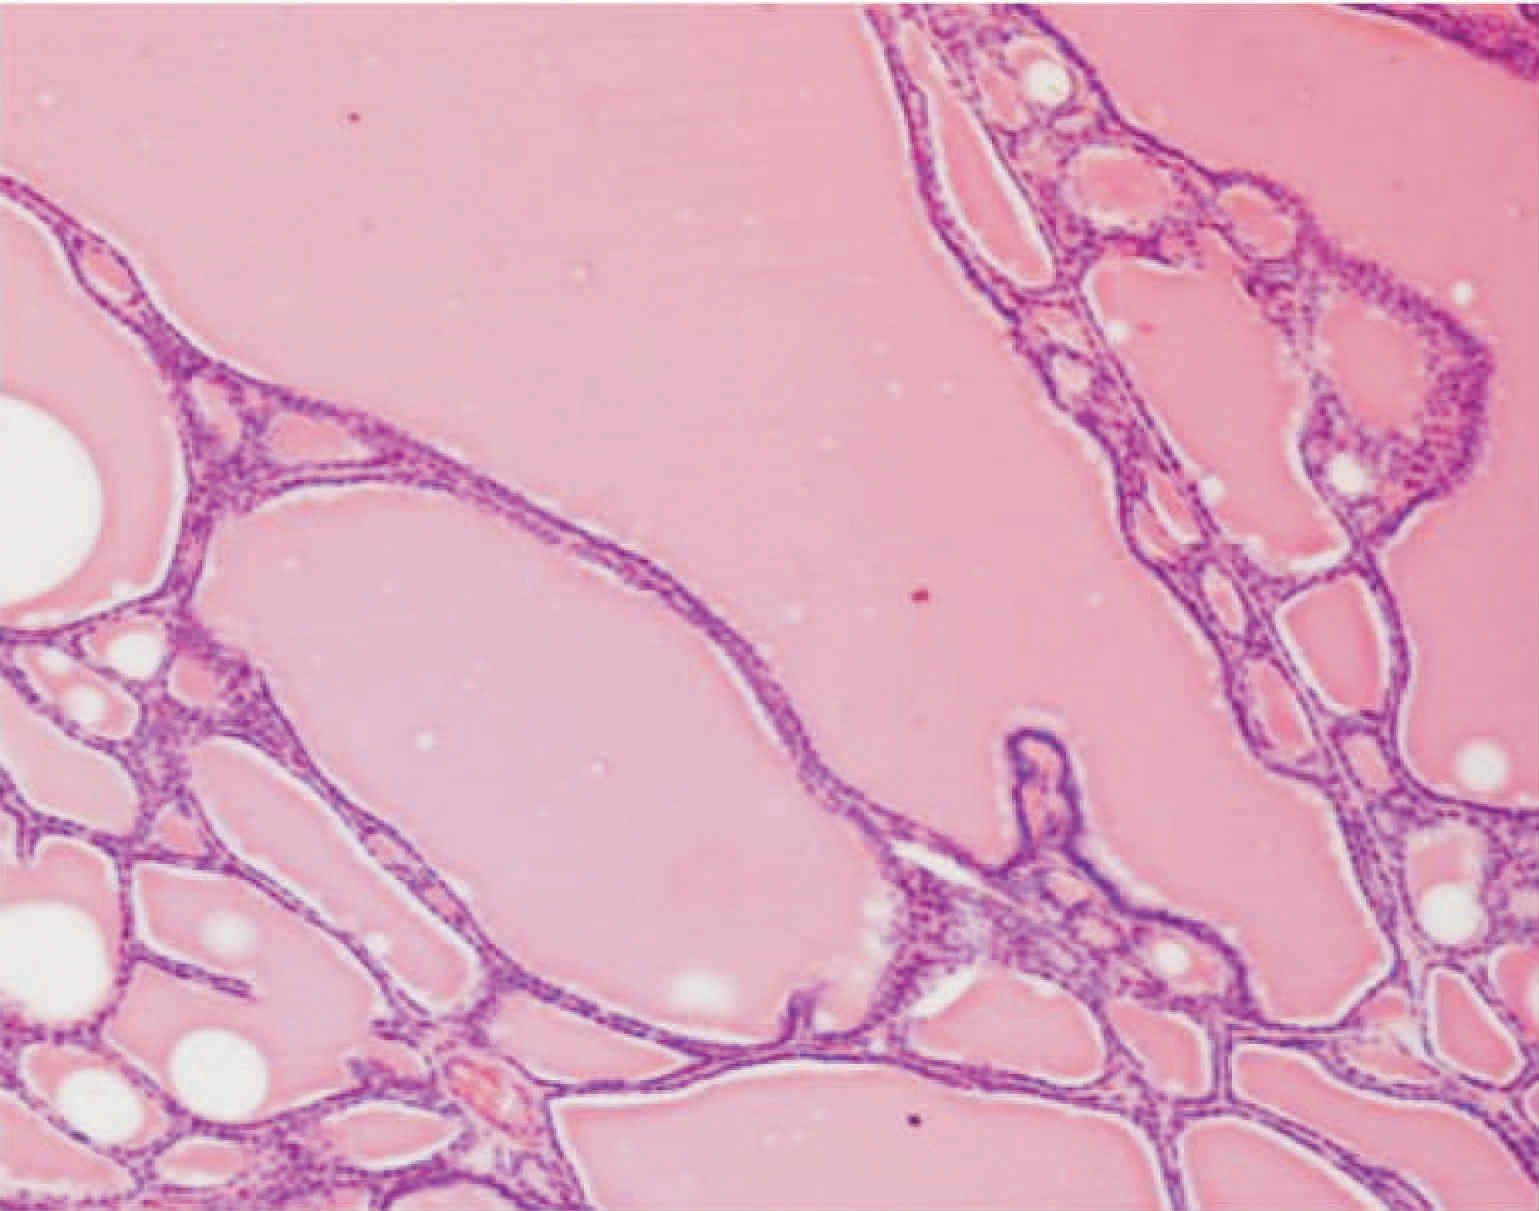
\includegraphics{./images/Image00208.jpg}
 \captionsetup{justification=centering}
 \caption{单纯性甲状腺肿(胶质贮积期,HE染色,低倍)}
 \label{fig12-1}
	\end{minipage}
	%	\end{figure} 
	%\FloatBarrier
	%\begin{figure}[!htbp]
	%    \centering
	\hspace{0.04\textwidth}%
	\begin{minipage}[b]{0.45\textwidth}
		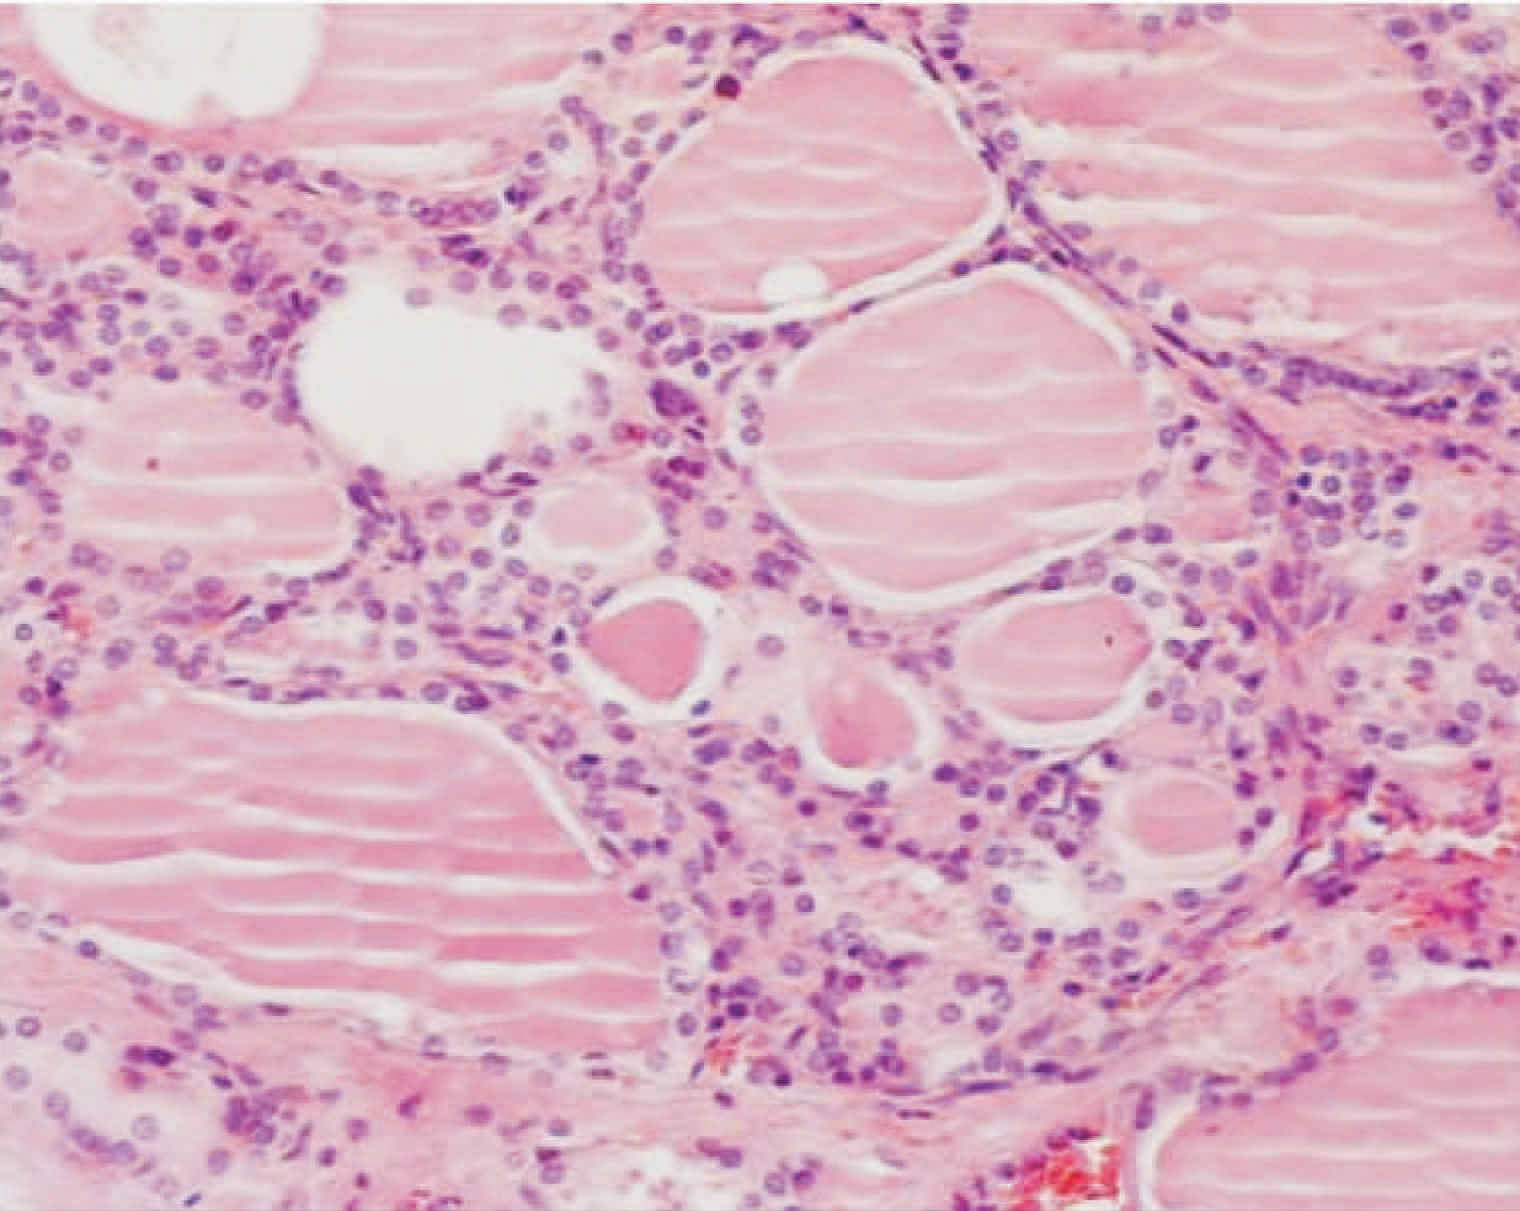
\includegraphics{./images/Image00209.jpg}
 \captionsetup{justification=centering}
 \caption{单纯性甲状腺肿(结节期,HE染色,中倍)}
 \label{fig12-2}
	\end{minipage}
\end{figure}

\subsection{弥漫性毒性甲状腺肿}

弥漫性毒性甲状腺肿(diffuse toxic
goiter)是一种自身免疫性疾病,临床表现并不限于甲状腺,而是一种多系统的临床综合征,包括高代谢症候群、弥漫性甲状腺肿、眼征、皮损和甲状腺肢端病。由于多数患者同时有高代谢症和甲状腺肿大,故称为弥漫性毒性甲状腺肿,又称Graves病,亦有弥漫性甲状腺肿伴功能亢进症、突眼性甲状腺肿、原发性甲状腺肿伴功能亢进症、Basedow病等之称。临床上主要表现为甲状腺肿大,基础代谢率和神经兴奋性升高,T3、T4高,吸碘率高,心悸、多汗、烦热、脉搏快、手震颤、多食、消瘦、乏力、突眼等。本病多见于女性,男女之比为1∶4~6,以20~40岁最多见。

\subsubsection{病因及发病机制}

目前一般认为本病与下列因素有关:

\paragraph{免疫系统异常}
本病为自身免疫性疾病,其根据:一是血中球蛋白增高,并有多种抗甲状腺的自身抗体,且常与一些自身免疫性疾病并存;二是血中存在与TSH受体结合的抗体,具有类似TSH的作用。

\paragraph{遗传因素}
家族中常可见到先后发病的病例,且多为女性。约有15%的患者有明显的遗传因素。患者的亲属约有一半血中存在甲状腺自身抗体。甲亢的发生与人白细胞抗原(HLAⅡ类抗原)显著相关。

\paragraph{精神创伤}
各种原因导致的精神过度兴奋,或过度抑郁,均可导致甲状腺激素的过度分泌,其机制可能是高度应激时肾上腺皮质激素的分泌急剧升高从而改变抑制性T淋巴细胞(Ts)或辅助性T淋巴细胞(Th)的功能,增强了免疫反应而促进自身免疫疾病的发生。

\subsubsection{病理变化}

肉眼观:甲状腺弥漫性对称性增大,为正常的2~4倍,表面光滑,血管充血,质地较软,切面呈分叶状灰红色,胶质少,质如肌肉。镜下观:①滤泡上皮增生呈高柱状,有的呈乳头样增生,并有小滤泡形成;②滤泡腔内胶质稀薄,滤泡周边胶质出现许多大小不一的上皮细胞的吸收空泡(图\ref{fig12-3});③间质血管丰富、充血,淋巴组织增生。电镜下:滤泡上皮细胞浆内质网丰富、扩张,高尔基体肥大、核糖体增多,分泌活跃。免疫荧光:滤泡基底膜上有IgG沉着。甲亢手术前往往须经碘治疗,治疗后甲状腺病变有所减轻,甲状腺体积缩小,质变实,镜下观见上皮细胞变矮,增生减轻,胶质增多变浓,吸收空泡减少,间质血管减少,充血减轻,淋巴细胞也减少。

\begin{figure}[!htbp]
 \centering
 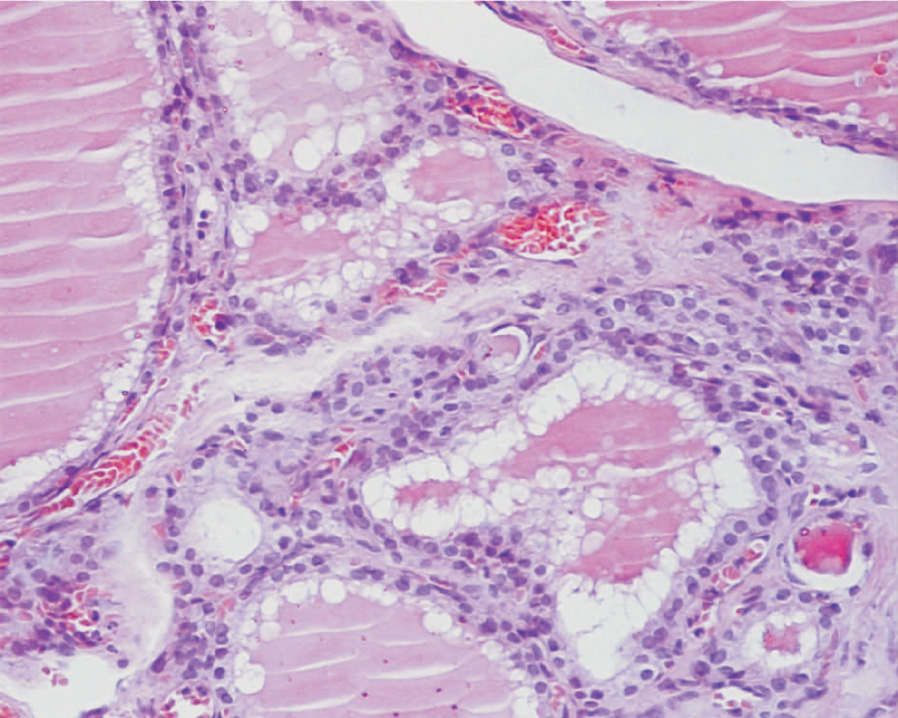
\includegraphics{./images/Image00210.jpg}
 \captionsetup{justification=centering}
 \caption{弥漫性毒性甲状腺肿(HE染色,高倍)\\ {\small 滤泡上皮增生,腔内胶质稀薄,滤泡周边胶质出现吸收空泡;间质血管丰富、充血}}
\label{fig12-3}
  \end{figure}

除甲状腺病变外,全身可有淋巴组织增生、胸腺和脾脏增大,心脏肥大、扩大,心肌和肝细胞可有变性、坏死及纤维化。眼球外突的原因是眼球外肌水肿、球后纤维脂肪组织增生、淋巴细胞浸润和黏液水肿。

\subsection{甲状腺肿瘤}

甲状腺发生的肿瘤和瘤样病变种类较多,组织学分类也不一致,现就常见的甲状腺肿瘤进行简要介绍。

\subsubsection{甲状腺腺瘤}

甲状腺腺瘤(thyroid
adenoma)是起源于甲状腺滤泡上皮的一种常见的良性肿瘤,好发于甲状腺功能的活动期,患者往往在无意中发现,中青年女性多见。肿瘤生长缓慢,随吞咽活动而上下移动。肉眼观:多为单发,圆或类圆形,直径一般3~5
cm,切面多为实性,色暗红或棕黄,可并发出血、囊性变、钙化和纤维化。有完整的包膜,常压迫周围组织。根据肿瘤组织形态学特点分类分别介绍如下:

\paragraph{单纯型腺瘤(simple adenoma)}
又称正常大小滤泡型腺瘤(normol-follicular
adenoma),肿瘤包膜完整,肿瘤组织由大小较一致、排列拥挤、内含胶质、与成人正常甲状腺相似的滤泡构成(图\ref{fig12-4})。

\paragraph{胶样型腺瘤(colloid adenoma)}
又称巨滤泡型腺瘤(macrofollicular
adenoma),肿瘤组织由大滤泡或大小不一的滤泡组成,滤泡内充满胶质,并可互相融合成囊。肿瘤间质少(图\ref{fig12-4})。

\begin{figure}[!htbp]
 \centering
 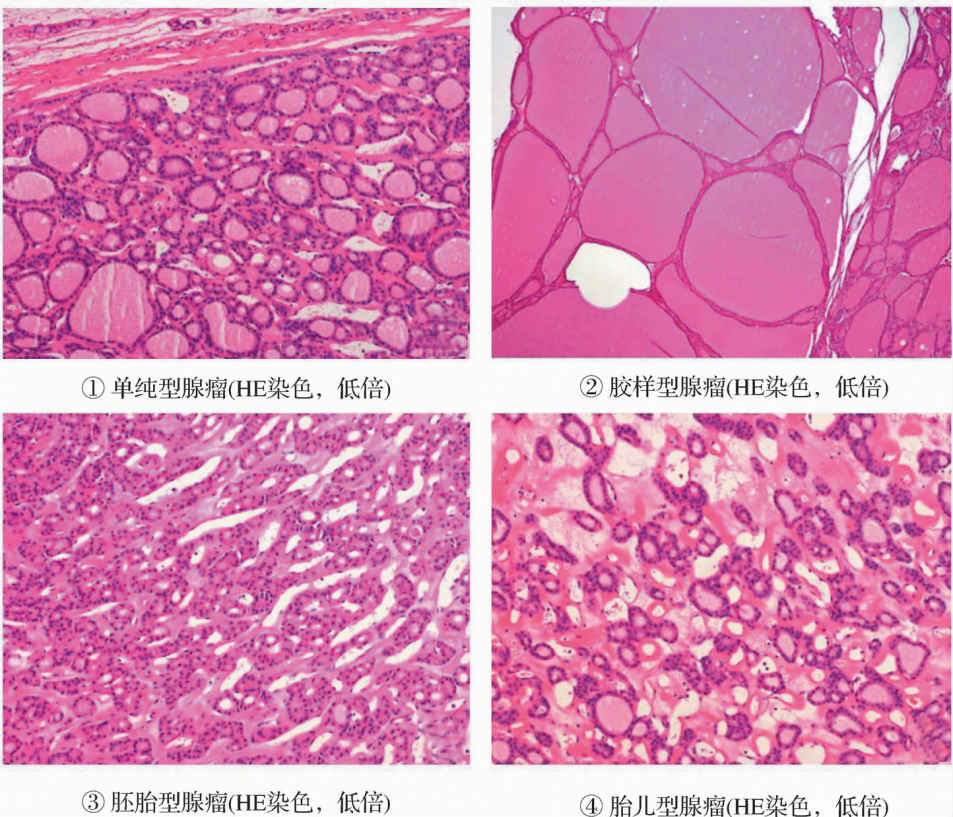
\includegraphics{./images/Image00211.jpg}
 \captionsetup{justification=centering}
 \caption{甲状腺腺瘤组织形态}
 \label{fig12-4}
  \end{figure} 

\paragraph{胚胎型腺瘤(embryonal adenoma)}
又称梁状和实性腺瘤(trabecular
and solid
adenoma),瘤细胞小,大小较一致,分化好,呈片状或条索状排列,偶见不完整的小滤泡,无胶质,间质疏松呈水肿状(图\ref{fig12-4})。

\paragraph{胎儿型腺瘤(fetal adenoma)}
又称小滤泡型腺瘤(microfollicular
adenoma),主要由小而一致、仅含少量胶质或没有胶质的小滤泡构成,上皮细胞为立方形,似胎儿甲状腺组织(图\ref{fig12-4}),间质呈水肿、黏液样,此型易发生出血、囊性变。

\paragraph{嗜酸细胞型腺瘤(acidophilic cell type adenoma)}
又称
Hürthle(许特莱)细胞腺瘤。较少见,瘤细胞大而多角形,核小,胞浆丰富嗜酸性,内含嗜酸性颗粒。电镜下见嗜酸性细胞内有丰富的线粒体,即Hürthle细胞。瘤细胞排列成索网状或巢状,很少形成滤泡。

\paragraph{非典型腺瘤(atypical adenoma)}
瘤细胞丰富,生长较活跃,有轻度非典型增生,可见核分裂象。瘤细胞排列成索或巢片状,很少形成完整滤泡,间质少,但无包膜和血管侵犯。本瘤应追踪观察,并与甲状腺髓样癌和转移癌鉴别,可作降钙素(calcitonin)、上皮膜抗原(epithelial
membrane
antigen,EMA)和角蛋白(keratin)等免疫组织化学检查,髓样癌Calcitonin阳性,转移癌EMA、keratin等阳性。

\subsubsection{甲状腺癌}

甲状腺癌(thyroid
carcinoma)是一种较常见的恶性肿瘤,约占所有恶性肿瘤的1%,约占甲状腺原发性上皮性肿瘤的1/3,男女之比约2∶3,任何年龄均可发生,但以40~50岁多见。多数甲状腺癌患者甲状腺功能正常,仅少数引起甲状腺功能亢进或低下。根据肿瘤组织形态学特点将甲状腺癌分为4种。

\paragraph{乳头状癌(papillary carcinoma)}
最常见的类型,约占60%,青少年、女性多见,约为男性的3倍,肿瘤生长慢,恶性程度较低,预后较好,10年存活率达80%以上。肉眼观:肿瘤一般为圆形,直径为2~3
cm,无包膜,质地较硬,切面灰白,常伴有出血、坏死、纤维化和钙化。镜下观:乳头分枝多,乳头中心有纤维血管间质,间质内常见呈同心圆状的钙化小体,即砂砾体(psammoma
bodies)(图\ref{fig12-5}),有助于诊断。乳头上皮可呈单层或多层,癌细胞可分化程度不一,核染色质少,常呈透明或毛玻璃状,无核仁。

\begin{figure}[!htbp]
 \centering
 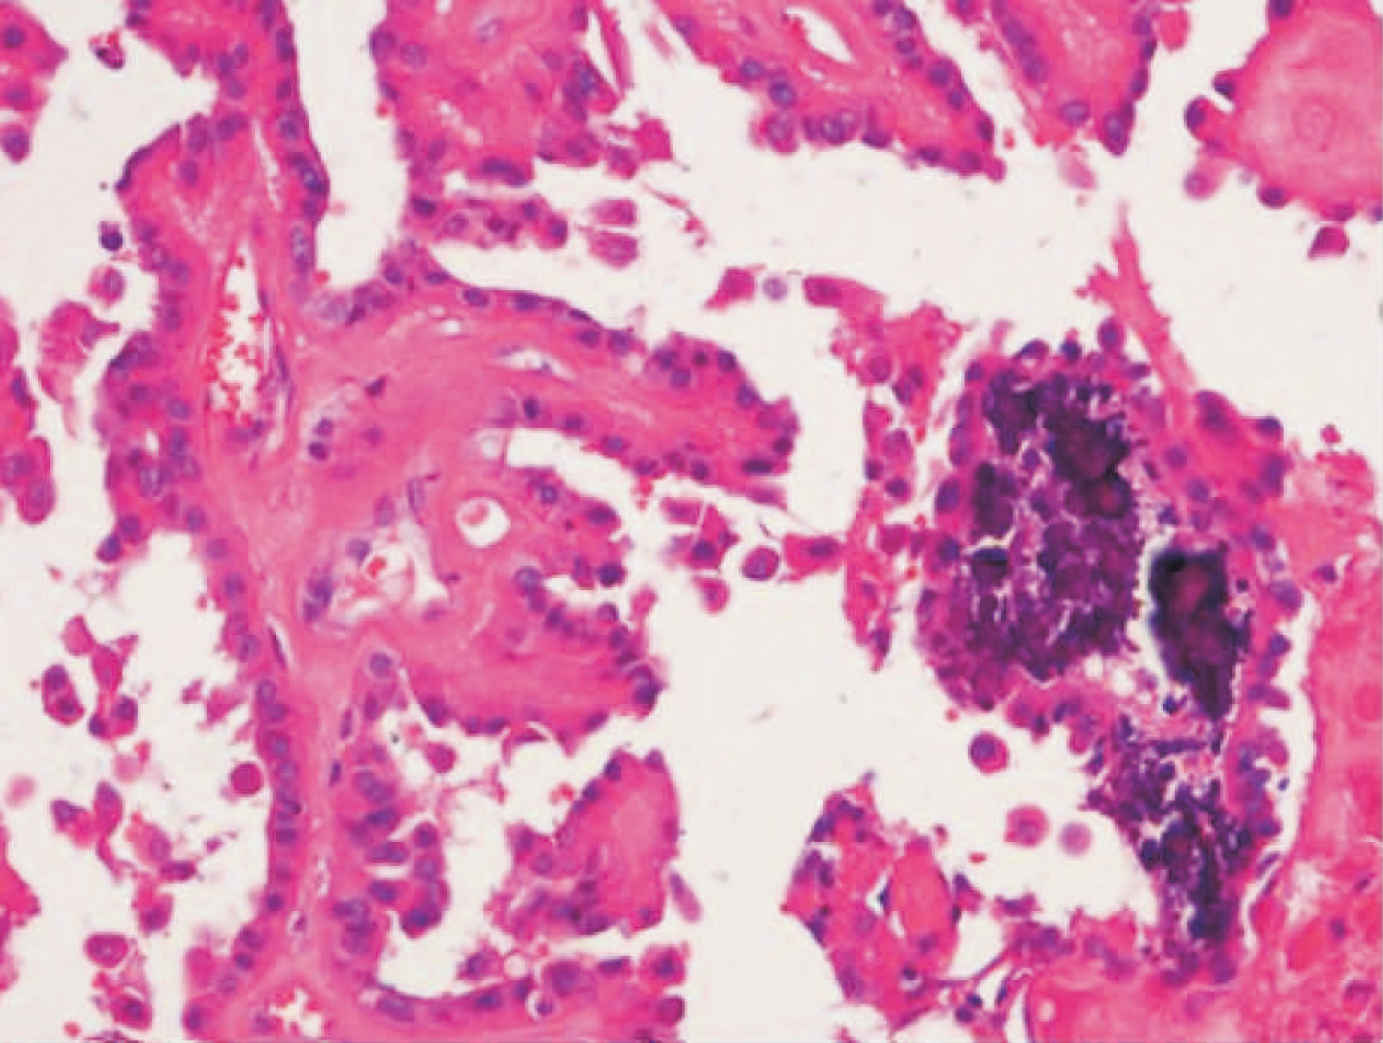
\includegraphics{./images/Image00212.jpg}
 \captionsetup{justification=centering}
 \caption{甲状腺乳头状癌(HE染色,中倍)\\ {\small 局部钙盐沉积,形成砂砾体}}
\label{fig12-5}
  \end{figure}

\paragraph{滤泡癌(follicular carcinoma)}
一般比乳头状癌恶性程度高、预后差,较常见,仅次于甲状腺乳头状癌而居第2位。多发于40岁以上女性,早期易发生血道转移,癌组织侵犯周围组织或器官时可引起相应的症状。肉眼观:结节状,包膜不完整,境界较清楚,切面灰白、质软。镜下观:可见不同分化程度的滤泡,有时分化好的滤泡癌很难与腺瘤区别,须多处取材、切片,注意是否有包膜和血管侵犯加以鉴别;分化差的呈实性巢片状,瘤细胞异型性明显,滤泡少而不完整(图\ref{fig12-6})。

\begin{figure}[!htbp]
 \centering
 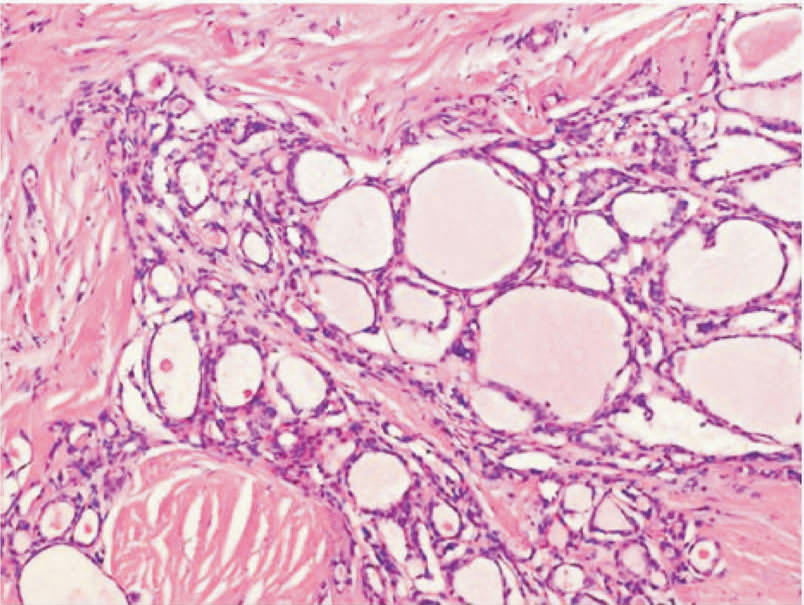
\includegraphics{./images/Image00213.jpg}
 \captionsetup{justification=centering}
 \caption{甲状腺滤泡癌(HE染色,低倍)\\ {\small 癌性滤泡侵犯包膜}}
\label{fig12-6}
  \end{figure}

\paragraph{髓样癌(medullary carcinoma)}
又称C细胞癌(C-cell
carcinoma),是由滤泡旁细胞(即C细胞)发生的恶性肿瘤,占甲状腺癌的5%~10%,40~60岁为高发期,部分为家族性常染色体显性遗传,90%的肿瘤分泌降钙素,产生严重腹泻和低钙血症,有的还同时分泌其他多种激素和物质。肉眼观:单发或多发,可有假包膜,直径1~11
cm,切面灰白或黄褐色,质实而软。镜下观:瘤细胞圆形或多角、梭形,核圆或卵圆,核仁不明显。瘤细胞呈实体片巢状或乳头状、滤泡状排列,间质内常有淀粉样物质沉着(可能与降钙素分泌有关)。

\paragraph{未分化癌(undifferentiated carcinoma)}
又称间变性癌(anaplastic
carcinoma)或肉瘤样癌(sarcomatoid
carcinoma),较少见,多发生在50岁以上,女性较多见,生长快,早期即可发生浸润和转移,恶性程度高,预后差。肉眼观:肿块较大,病变不规则,无包膜,广泛浸润、破坏,切面灰白,常有出血、坏死。镜下观:癌细胞大小、形态、染色深浅不一,核分裂象多。组织学上可分为小细胞型、梭形细胞型、巨细胞型和混合细胞型。

\section{糖尿病}

\begin{framed}
{案例12-2}

{【病例摘要】}

患者,男,59岁,多饮多食多尿,消瘦,易感染,血糖升高多年,曾间断性服用降糖药,近期出现肾衰竭,失明。

{【问题】}

1. 请做出诊断并提出诊断依据。

2. 试述胰岛、血管、肾脏、视网膜病变。
\end{framed}

糖尿病(diabetes
mellitus)是一种体内胰岛素相对或绝对不足或靶细胞对胰岛素敏感性下降,或胰岛素本身存在结构上的缺陷而引起的碳水化合物、脂肪和蛋白质代谢紊乱的一种慢性疾病。其主要特点是高血糖和糖尿。临床上典型表现为多饮、多食、多尿和体重减少(即“三多一少”),糖尿病时长期存在的高血糖,导致各组织,特别是眼、肾、心脏、血管、神经的慢性损害、功能障碍。本病发病率日益增高,已成为世界性的常见病、多发病。

\subsection{分类}

糖尿病一般分为原发性糖尿病(primary diabetes
mellitus)和继发性糖尿病(secondary diabetes
mellitus)。原发性糖尿病(即日常所俗称的糖尿病)又分为胰岛素依赖型糖尿病(insulin-dependent
diabetes mellitus,IDDM)和非胰岛素依赖型糖尿病(non-insulin-dependent
diabetes
mellitus,NIDDM)两种。继发性糖尿病,指已知原因造成胰岛内分泌功能不足所致的糖尿病。

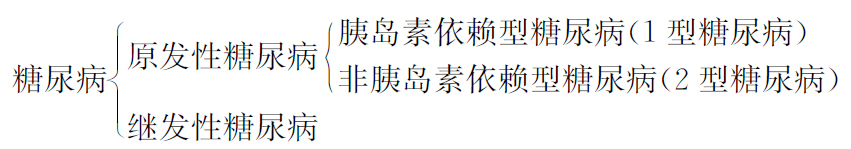
\includegraphics{./images/Image00214.jpg}

\subsection{病因及发病机制}

不同类型的糖尿病其病因和发病机制不尽相同。

\paragraph{原发性糖尿病}
(1)胰岛素依赖型:又称1型糖尿病,约占糖尿病的10%,多发生在儿童和青少年,起病急,病情重,进展快,胰岛B细胞严重受损,细胞数目明显减少,胰岛素分泌绝对不足,血中胰岛素降低,引起糖尿病,易出现酮症,治疗依赖胰岛素。目前认为本型是在遗传易感性的基础上由病毒感染等诱发的针对B细胞的一种自身免疫性疾病。

(2)非胰岛素依赖型:又称2型糖尿病,多发生于成年人,肥胖者多见,多在35~40岁之后发病,占糖尿病患者90%以上。起病缓慢,病情较轻,发展较慢,不易出现酮症,胰岛数目正常或轻度减少,2型糖尿病患者体内产生胰岛素的能力并非完全丧失,有的患者体内胰岛素甚至产生过多,但胰岛素的作用效果较差,因此患者体内的胰岛素是一种相对缺乏,可以通过某些口服药物刺激体内胰岛素的分泌,一般可以不依赖胰岛素治疗。本型病因、发病机制不清楚,认为是与遗传、环境、年龄、种族、生活方式等有关的胰岛素相对不足及组织对胰岛素不敏感所致。

\paragraph{继发性糖尿病}
指已知原因造成胰岛内分泌功能不足所致的糖尿病,如炎症、肿瘤,手术或其他损伤和某些内分泌疾病(如肢端肥大症、Cushing综合征、甲亢、嗜铬细胞瘤和类癌综合征)等。

不同类型糖尿病造成的长期并发症相同,其发生机制极为复杂。持续高血糖是关键,而糖基化终产物形成、炎症因子释放、自由基产生增多、蛋白激酶C激活和多元醇通路紊乱等均与发病有关。

\subsection{病理变化}

糖尿病的损害并不仅仅局限于胰岛,而是累及多器官多系统。

\paragraph{胰岛病变}
不同类型、不同时期病变不同。1型糖尿病早期为非特异性胰岛炎,继而胰岛B细胞颗粒脱失、空泡变性、坏死、消失,胰岛变小、数目减少,纤维组织增生、玻璃样变;2型糖尿病早期病变不明显,后期B细胞减少,常见胰岛淀粉样变性(图\ref{fig12-7})。

\begin{figure}[!htbp]
 \centering
 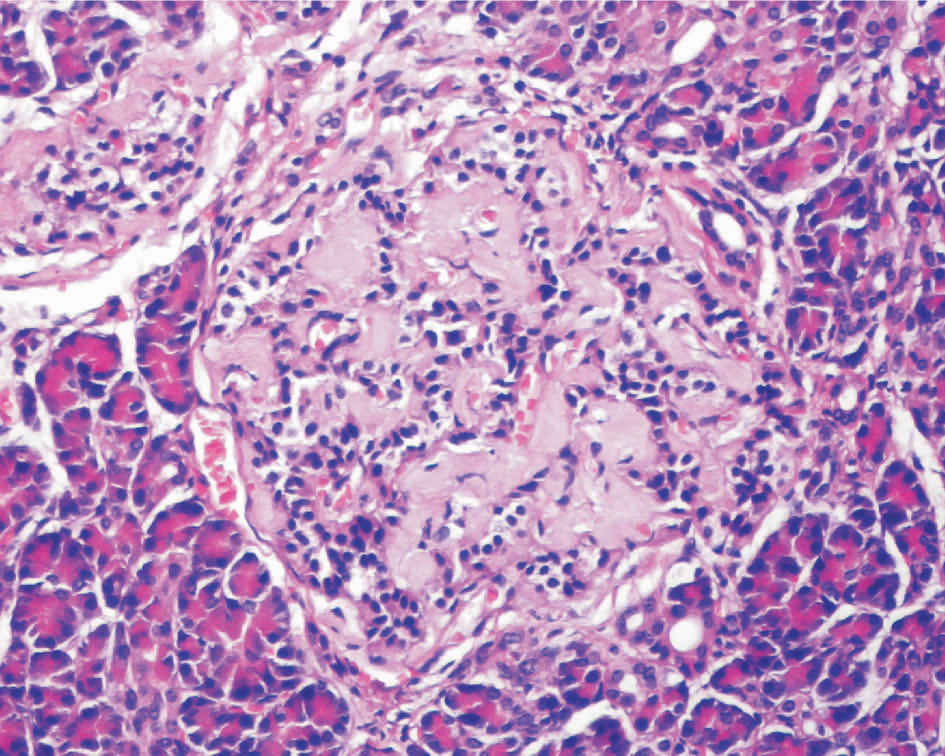
\includegraphics{./images/Image00215.jpg}
 \captionsetup{justification=centering}
 \caption{2型糖尿病胰岛淀粉样变性(HE染色,中倍)}
 \label{fig12-7}
  \end{figure} 

\paragraph{血管病变}
糖尿病病人从毛细血管到大中动脉均可有不同程度的病变,且病变发病率较一般人群高,发病早,病变严重。

(1)毛细血管和细、小动脉:毛细血管和细、小动脉内皮细胞增生,基底膜明显增厚,有的比正常厚几倍乃至十几倍,血管壁增厚、玻璃样变性、变硬,血压增高;有的血管壁发生纤维素样变性和脂肪变性,血管壁通透性增强;有的可有血栓形成或管腔狭窄,导致血液供应障碍,引起相应组织或器官缺血、功能障碍和病变。电镜下:内皮细胞增生,基底膜高度增厚,有绒毛样突起,突向管腔,内皮细胞间联结增宽,可见窗孔形成,内皮细胞饮液小泡增加,有的管壁有纤维素样坏死,有的地方有血小板聚集,血栓形成。

(2)大、中动脉:大、中动脉有动脉粥样硬化或中层钙化,粥样硬化病变程度重。临床表现为主动脉、冠状动脉、下肢动脉、脑动脉和其他脏器动脉粥样硬化,引起冠心病、心肌梗死、脑萎缩、肢体坏疽等。

\paragraph{肾脏病变}
(1)肾脏体积增大:由于糖尿病早期肾血流量增加,肾小球滤过率增高,导致早期肾脏体积增大,通过治疗可恢复正常。

(2)结节性肾小球硬化:表现为肾小球系膜内有结节状玻璃样物质沉积,即K-W结节,结节增大可使毛细血管腔阻塞(图\ref{fig12-8})。

(3)弥漫性肾小球硬化:约见于75%的病人,同样在肾小球内有玻璃样物质沉积,分布弥漫,主要损害肾小球毛细血管壁和系膜,肾小球基底膜普遍增厚,毛细血管腔变窄或完全闭塞,最终导致肾小球缺血和玻璃样变性。

(4)肾小管---间质性损害:肾小管上皮细胞出现颗粒样和空泡样变性(属退行性变),晚期肾小管萎缩。肾间质病变包括纤维化、水肿和淋巴细胞、浆细胞和多形核白细胞浸润。

(5)血管损害:糖尿病累及所有的肾血管,多数损害的是肾动脉,引起动脉硬化,特别是入球和出球小动脉硬化。至于肾动脉及其主要分支的动脉粥样硬化,在糖尿病人要比同龄的非糖尿病人出现得更早、更常见。

(6)肾乳头坏死:常见于糖尿病人患急性肾盂肾炎时,肾乳头坏死是缺血并感染所致。

\begin{figure}[!htbp]
 \centering
 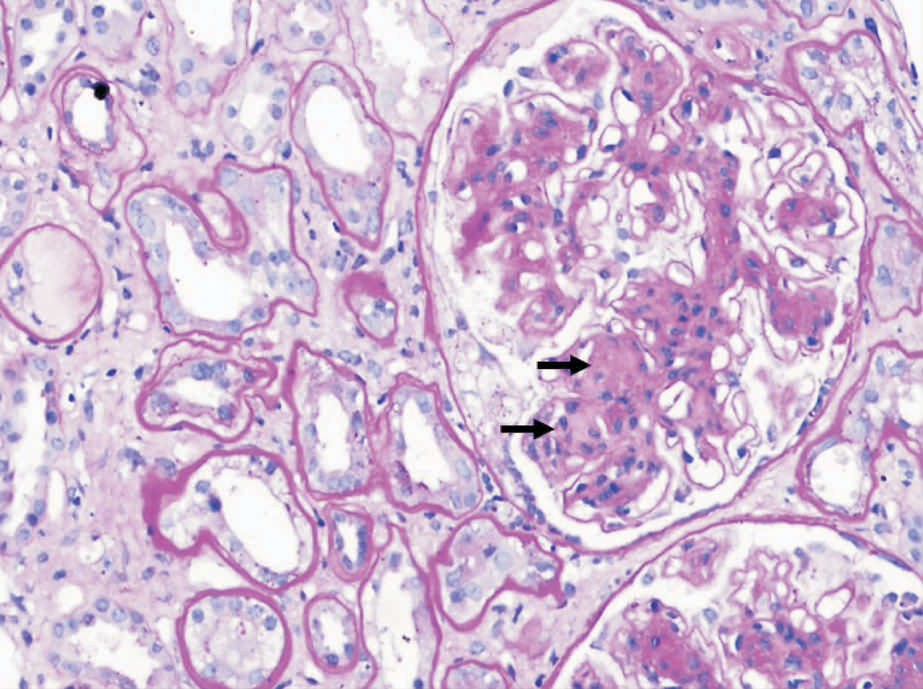
\includegraphics{./images/Image00216.jpg}
 \captionsetup{justification=centering}
 \caption{糖尿病肾病(PAS染色,中倍)\\ {\small 结节性肾小球硬化,K-W结节形成(箭头所示);肾小管基底膜增厚;肾间质增生}}
\label{fig12-8}
  \end{figure}

\paragraph{视网膜病变}
早期表现为微小动脉瘤和视网膜小静脉扩张,继而渗出、水肿、微血栓形成、出血等非增生性视网膜病变。还可因血管病变引起缺氧,刺激纤维组织增生、新生血管形成等增生性视网膜性病变。视网膜病变可造成白内障或失明。

\paragraph{神经系统病变}
周围神经可因血管病变引起缺血性损伤或症状,如肢体疼痛、麻木、感觉丧失、肌肉麻痹等,脑细胞也可发生广泛变性。

\paragraph{其他组织或器官病变}
可出现皮肤黄色瘤、肝脂肪变和糖原沉积、骨质疏松、糖尿病性外阴炎及化脓性和真菌性感染等。

\begin{center}
    \textbf{知识链接}
\end{center}
\chapterabstract{目前尚无根治糖尿病的方法,但通过多种治疗手段可以控制好糖尿病。主要包括5个方面,通常称之为糖尿病治疗的五驾马车,即:糖尿病患者的健康教育、自我监测血糖、饮食治疗、运动治疗和药物治疗。

1. 健康教育

教育糖尿病患者懂得糖尿病的基本知识,树立战胜疾病的信心,如何控制糖尿病,控制好糖尿病对健康的益处。根据每个糖尿病患者的病情特点制定恰当的治疗方案。

2. 自我监测血糖

随着小型快捷血糖测定仪的逐步普及,病人可以根据血糖水平随时调整降血糖药物的剂量。1型糖尿病进行强化治疗时每天至少监测4次血糖(餐前),血糖不稳定时要监测8次(三餐前后、晚睡前和凌晨3:00)。

3. 药物治疗

目前糖尿病治疗的药物主要有磺脲类药物、双胍类、α葡萄糖苷酶抑制剂、胰岛素增敏剂、格列奈类和胰岛素。

4. 运动治疗

增加体力活动可改善机体对胰岛素的敏感性,降低体重,减少身体脂肪量,增强体力,提高工作能力和生活质量。运动的强度和时间长短应根据病人的总体健康状况来定,运动形式可多样,如散步、快步走、健美操、跳舞、打太极拳、跑步、游泳等。

5. 饮食治疗

饮食治疗是各种类型糖尿病治疗的基础,一部分轻型糖尿病患者单用饮食治疗就可控制病情。}

\section*{复习与思考}

{一、名词解释}

单纯性甲状腺肿 弥漫性毒性甲状腺肿 砂砾体 糖尿病

{二、思考题}

1. 试述弥漫性非毒性甲状腺肿的病理变化。

2. 试述糖尿病血管的病理变化。